\begin{figure}[t]
\centering
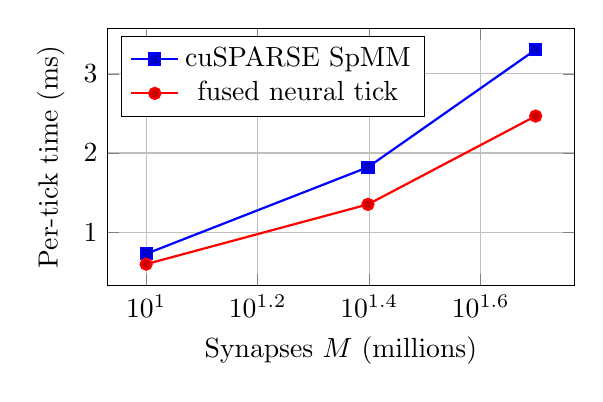
\begin{tikzpicture}
\begin{axis}[width=0.62\textwidth, height=0.4\textwidth, xlabel={Synapses $M$ (millions)}, ylabel={Per-tick time (ms)}, grid=both, xmode=log, legend pos=north west]
\addplot+[mark=square*, thick] coordinates {(10.00,0.725) (24.99,1.820) (49.95,3.305)};
\addplot+[mark=*, thick] coordinates {(10.00,0.595) (24.99,1.350) (49.95,2.466)};
\legend{cuSPARSE SpMM, fused neural tick}
\end{axis}
\end{tikzpicture}
\caption{Fixed-topology tick cost against a same-parameter cuSPARSE multiplication (RTX 5070 Laptop, batch 1). The complete neural update is cheaper than the library denominator because it fuses the elementwise work.}
\label{fig:tick}
\end{figure}
